% ==========================================================
\section{Existing GLSP-Based Diagram Editors}
\label{sec:sota_glsp}
% ==========================================================
 
To understand the practical scope of \gls{glsp} and the architectural conventions that have emerged around it, this section examines concrete tools and applications built on top of the framework.
First, the reference implementations maintained by the \gls{glsp} project are described; these establish baseline patterns and best practices.
Next, BigUML is analyzed as a more ambitious third-party tool that stress-tests the framework's ability to scale to complex, multi-diagram specifications.
The section closes with a discussion of a prototype that extends \gls{glsp}'s protocol and architecture to support real-time collaborative modeling, illustrating the framework's extensibility for novel use cases.
 
% ----------------------------------------------------------
\subsection{Example Projects of the GLSP maintainers}
\label{subsec:glsp_examples}
% ----------------------------------------------------------
 
\paragraph{Server and client frameworks.}
To lower barriers to entry for \gls{glsp} users, the project provides two production-ready server implementations alongside its client library.
The Java server framework integrates tightly with the Eclipse Modeling Framework (EMF), enabling developers to leverage existing metamodels and model manipulation logic without reimplementation~\cite{noauthor_eclipse-glspglsp-server_2026}.
The TypeScript server framework, in contrast, executes natively on Node.js and enables a homogeneous full-stack development experience when combined with the TypeScript client~\cite{noauthor_eclipse-glspglsp-server-node_2026}.
 
On the client side, \gls{glsp} builds upon Eclipse Sprotty~\cite{noauthor_eclipse-sprottysprotty_2026}, a mature graphics library that transforms abstract graph models into interactive SVG visualizations rendered in the browser.
Crucially, \gls{glsp} extends Sprotty's base graph schema (\texttt{SGraph}) into its own \texttt{GModel} while deliberately preserving direct access to the underlying SVG and CSS rendering layer~\cite{bork_vision_2024}.
This design choice grants tool developers complete control over the visual representation of shapes, connectors, and interaction behaviors, enabling high degrees of customization without the need to fork the framework.
 
For deployment and integration, \gls{glsp} employs a clear architectural separation between platform-independent editor logic and host-application-specific concerns through dedicated integration modules.
Platform-specific adapter packages enable the same diagram editor to be deployed into Eclipse RCP~\cite{noauthor_eclipse-glspglsp-eclipse-integration_2026}, VS Code~\cite{noauthor_eclipse-glspglsp-vscode-integration_2026}, Eclipse Theia~\cite{noauthor_eclipse-glspglsp-theia-integration_2026}, or any plain web application~\cite{noauthor_eclipse-glspglsp-client_2026}.
This approach allows developers to reuse the same core editor logic and diagram definitions across multiple targets~\cite{bork_vision_2024}.
Moreover, the Node.js server implementation enables developers to run \gls{glsp} fully in the browser~\cite{bork_vision_2024}.
 
\paragraph{The Workflow Diagram example.}
The primary reference implementation for \gls{glsp} is the Workflow Diagram example~\cite{noauthor_eclipse-glspglsp-examples_2026}.
It is a simplified flow-chart editor designed to serve as the canonical demonstration of \gls{glsp}'s capability set.
The example implementation includes the usage of all previously described server frameworks and client integrations.
The workflow diagram showcases a comprehensive set of node and edge types, interaction patterns, and editor features that collectively exercise the full range of \gls{glsp}'s architectural capabilities.
The example is fully open-source, explicity functioning as a blueprint for custom implementations, allowing developers to understand both \gls{glsp} architecture and best practices through a single, authoritative example.

\begin{figure}[ht]
    \centering
    \begin{subfigure}[t]{0.49\textwidth}
        \centering
        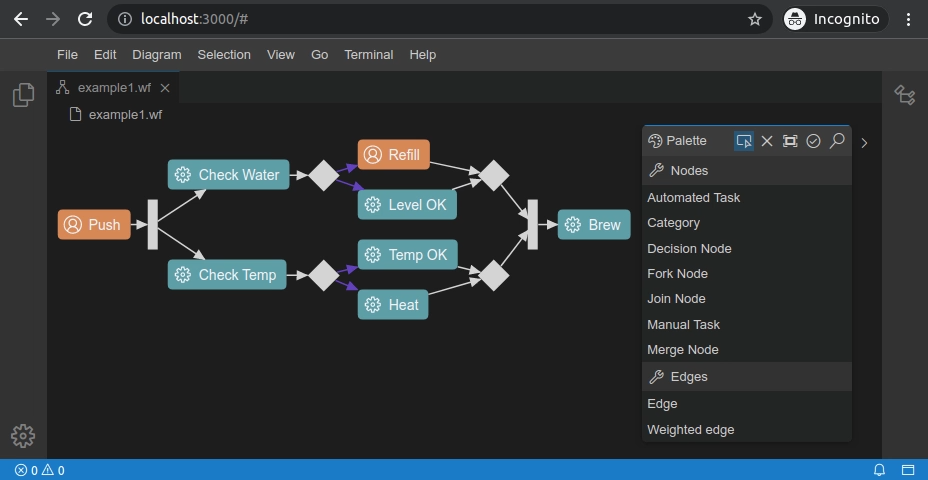
\includegraphics[width=\linewidth]{figures/glsp-workflow.png}
        \caption{Workflow diagram. Taken from~\cite{noauthor_eclipse-glspglsp_2026}.}
        \label{fig:glsp_workflow}
    \end{subfigure}
    \hfill
    \begin{subfigure}[t]{0.49\textwidth}
        \centering
        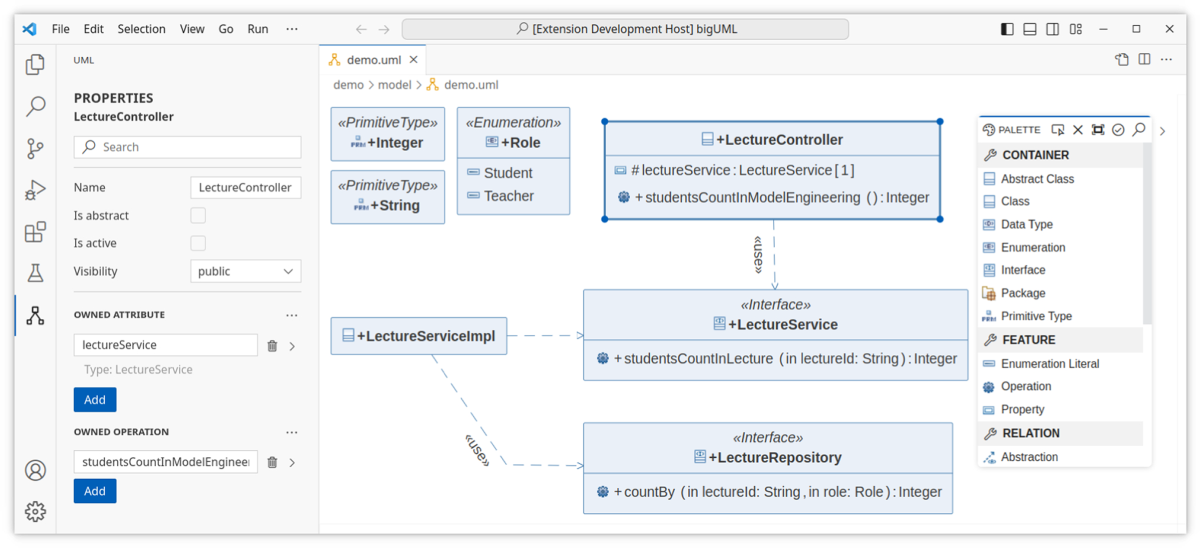
\includegraphics[width=\linewidth]{figures/big-uml.png}
        \caption{BigUML class diagram. Taken from \cite{metin_developing_2023}.}
        \label{fig:big_uml}
    \end{subfigure}
    \caption[Examples of GLSP projects]{Different examples of diagram editors based on the \gls{glsp} framework.}
    \label{fig:glsp_examples}
\end{figure}
 
% ----------------------------------------------------------
\subsection{BigUML}
\label{subsec:biguml}
% ----------------------------------------------------------
 
BigUML~\cite{metin_developing_2023} is a proof-of-concept UML modeling tool built on \gls{glsp} that validates the framework's viability for constructing large-scale, specification-driven diagram editors.
Implementing comprehensive web tooling for UML is notoriously demanding because the specification defines numerous structurally distinct diagram types, each with unique visual notations and semantic rules.
BigUML demonstrates that \gls{glsp} can meet this challenge while delivering advanced end-user features, all organized into a modular architecture of core services, tool-level features, and diagram-specific modules~\cite{metin_developing_2023}.
 
\paragraph{Source Model Representation Separation.}
The central architectural concept that allows BigUML to handle multiple UML diagram types over a shared source model is Source Model Representation Separation~\cite{metin_developing_2023}.
The same underlying model element may need to be rendered differently depending on which diagram type is currently active.
When a diagram is saved, BigUML persists the diagram's representation type, for example, a class diagram and a communication diagram, to the file system alongside the source model.
When the model is subsequently read, the model server supplies this representation identifier to the \gls{glsp} server, which uses it to load the correct language-specific diagram module.
User requests are then dispatched exclusively to that module, ensuring that distinct diagram representations share source data without interfering with each other's visual rules or behavioural constraints.

% ----------------------------------------------------------
\subsection{Real-Time Collaborative Modeling in GLSP}
\label{subsec:glsp_collaboration}
% ----------------------------------------------------------
 
Real-time collaborative modeling in \gls{glsp} has been achieved by extending the protocol and architecture to support multiple users interacting with the same diagram concurrently~\cite{hegedus_real-time_2023, helming_real-time_nodate}.
One such prototype uses Visual Studio Live Share as the data exchange layer and implements a single-server architecture: a designated host machine runs the authoritative \gls{glsp} server holding the current model state, while guest clients proxy their edits through the host.
When a guest performs an edit, their action is forwarded via Live Share to the host client, which proxies it to the server; the resulting model update is broadcast back to all participants.
Since only one model state ever exists at any time, costly merge algorithms such as operational transformation are unnecessary.
To maintain safe undo-redo semantics in this shared context, the server was extended with a \textit{CommandStackManager} that maintains independent command stacks per user (identified by Live Share subclient ID), enabling each participant to undo only their own actions without affecting others' work.

Rather than enforcing restrictive element-level locking, the system resolves conflicts by allowing the most recent operation to succeed, and mitigates unintentional interference through rich {visual awareness feedback.
These awareness cues are transmitted via a dedicated \textit{CollaborationAction} message type sent directly between clients, bypassing the server, and include: live mouse pointers with participant name labels, dashed viewport outlines showing each participant's current view, and color-coded selection indicators on shared elements using each participant's assigned Live Share color.
Usability studies with BigUML and the Workflow Diagram confirmed that the system scales well for typical collaborative group sizes, with session performance determined primarily by the rate of concurrent edits rather than by model size or complexity~\cite{hegedus_real-time_2023}.